Every serious decision in science and engineering has the same shape. We act in a
large state space with limited time, finite energy, and incomplete information.
A logistics network picks routes, a physicist studies many-body matter, and an
algorithm designer studies hardness. All three are solving constrained
optimization problems on a physical substrate.

This chapter builds that common language from first principles. The goal is not
a philosophical survey. The goal is operational clarity for the rest of the
thesis. We need a precise account of hardness, a precise map from optimization
to Hamiltonians, and a physically grounded explanation of why adiabatic methods
are controlled by spectral geometry.

\section{Reality}
\label{sec:ch2-reality}

Only one philosophical commitment is needed here. Mathematics is a model of
regularities in the world, not a replacement for the world.

The consequence is concrete. A complexity claim is meaningful only after the
model and resource accounting are fixed. If access to the input changes, if
precision demands change, or if control primitives change, then the same task
can move from easy to hard.

For this thesis, the modeling chain is
\begin{figure}[h]
\centering
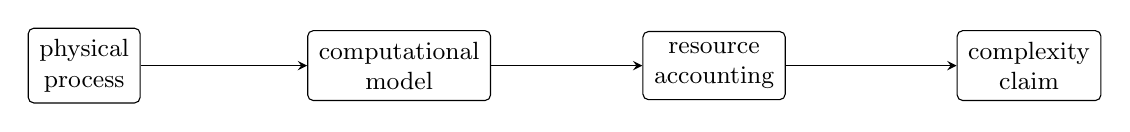
\begin{tikzpicture}[
  box/.style={draw, rounded corners=2pt, align=center, inner sep=4pt, font=\small},
  arr/.style={->, >=stealth, line width=0.5pt}
]
\node[box] (p) at (0,0) {physical\\process};
\node[box] (m) at (4.0,0) {computational\\model};
\node[box] (r) at (8.0,0) {resource\\accounting};
\node[box] (c) at (12.0,0) {complexity\\claim};
\draw[arr] (p) -- (m);
\draw[arr] (m) -- (r);
\draw[arr] (r) -- (c);
\end{tikzpicture}
\caption{Modeling chain used in this thesis: physical assumptions fix the
computational model, which fixes resource accounting, which supports complexity
claims.}
\label{fig:ch2-modeling-chain}
\end{figure}
Chapters 3 and 4 will follow this chain explicitly. The optimization objective
will be held fixed while the model shifts from query circuits to adiabatic
Hamiltonian evolution.

\section{Physics}
\label{sec:ch2-physics}

The Hamiltonian viewpoint unifies mechanics, thermodynamics, and optimization.
In classical mechanics, a Hamiltonian function generates dynamics by
\begin{equation}
\label{eq:ch2-hamilton-equations}
\dot{q}_j = \frac{\partial H_{\mathrm{cl}}}{\partial p_j},
\qquad
\dot{p}_j = -\frac{\partial H_{\mathrm{cl}}}{\partial q_j}.
\end{equation}

In statistical mechanics, low-energy preference appears as Gibbs weighting. For
cost profile $C(z)$ and inverse temperature $\beta=1/(k_B T)$,
\begin{equation}
\label{eq:ch2-gibbs}
\pi_\beta(z)=\frac{e^{-\beta C(z)}}{Z_\beta},
\qquad
Z_\beta=\sum_z e^{-\beta C(z)}.
\end{equation}
As $\beta \to \infty$, mass concentrates on minimizers of $C$.

Quantum mechanics keeps the Hamiltonian as generator, now as an operator on a
Hilbert space. Chapter 3 develops that formalism in detail. The key point here
is already visible. Energy is not just a physical observable. It is an
algorithmic objective function.

\section{Computation}
\label{sec:ch2-computation}

Computability and complexity separate what can be solved from what can be
solved efficiently. In the Turing model \cite{arora2009computational}, a
language $L\subseteq\{0,1\}^*$ is decidable if some Turing machine halts on
every input and accepts exactly strings in $L$.

The Church-Turing thesis concerns computability. The extended Church-Turing
thesis adds an efficiency claim, namely that physically realizable computation
is simulable by probabilistic classical computation with polynomial overhead
\cite{arora2009computational}. Quantum computation challenges this efficiency
extension while preserving computability.

The baseline decision classes are standard.

\begin{definition}[Class $\mathrm{P}$]
A decision problem is in $\mathrm{P}$ if a deterministic Turing machine solves
it in time polynomial in input length.
\end{definition}

\begin{definition}[Class $\mathrm{NP}$]
A decision problem is in $\mathrm{NP}$ if every yes-instance has a witness that
can be verified in polynomial time by a deterministic Turing machine.
\end{definition}

Hardness is transferred through reductions.

\begin{definition}[Polynomial-time many-one reduction]
For decision problems $A$ and $B$, write $A\leq_p B$ if there exists a
polynomial-time computable function $f$ such that
\begin{equation}
\label{eq:ch2-reduction}
x\in A \iff f(x)\in B.
\end{equation}
\end{definition}

\begin{definition}[NP-hard and NP-complete]
A problem $B$ is NP-hard if $A\leq_p B$ for every $A\in\mathrm{NP}$. If in
addition $B\in\mathrm{NP}$, then $B$ is NP-complete.
\end{definition}

SAT and 3-SAT are canonical hardness anchors \cite{Karp1972}. A 3-SAT formula
has the form
\begin{equation}
\label{eq:ch2-3sat}
F(x_1,\ldots,x_n)=\bigwedge_{j=1}^{m}(\ell_{j,1}\lor\ell_{j,2}\lor\ell_{j,3}),
\end{equation}
where each literal $\ell_{j,k}$ is either $x_i$ or $\overline{x}_i$.

Optimization enters this language through threshold decision. Given cost
function $C$ and threshold $\tau$, ask if there exists $z$ such that
$C(z)\leq\tau$. If that threshold language is NP-hard, generic exact
polynomial-time optimization is unlikely.

\section{The \texorpdfstring{$\#\mathrm{P}$}{\#P} Complexity Class}
\label{sec:ch2-sharpp}

Decision asks whether solutions exist. Many spectral tasks ask how many
solutions exist. That is a counting question.

\begin{definition}[Class $\#\mathrm{P}$]
A function $f:\{0,1\}^*\to\mathbb{N}$ is in $\#\mathrm{P}$ if there exists a
nondeterministic polynomial-time Turing machine $M$ such that $f(x)$ equals the
number of accepting branches of $M$ on input $x$.
\end{definition}

Valiant introduced this class and established hardness of canonical counting
problems \cite{valiant1979complexity}. The standard example is
\begin{equation}
\label{eq:ch2-sharpsat}
\#\mathrm{SAT}(F)=\left|\left\{x\in\{0,1\}^n : F(x)=1\right\}\right|.
\end{equation}
Decision SAT is recovered by testing whether this value is zero.

This distinction is structurally central in later chapters. The degeneracy
$d_0$ counts optimal configurations. Chapter 8 uses exactly this
decision-versus-counting split to separate NP-hard from
$\#\mathrm{P}$-hard precision regimes in spectral estimation.

\section{Linearity and Non-linearity}
\label{sec:ch2-linearity}

Physical laws are often locally linear in their state variables, while global
behavior is not. Small perturbations can trigger phase changes, metastability,
or abrupt spectral rearrangements.

Quantum evolution is linear in the state vector. With $\hbar=1$,
\begin{equation}
\label{eq:ch2-schrodinger-linear}
i\frac{d}{dt}\ket{\psi(t)}=H(t)\ket{\psi(t)}.
\end{equation}
The linearity of this equation does not imply linear computational difficulty.
Runtime depends on spectral geometry and available control resources.

This is the first major theme of the thesis. The interpolation law may look
simple, while the location and width of the relevant avoided crossing can depend
nonlinearly on the full spectrum of the problem Hamiltonian.

\section{Optimization}
\label{sec:ch2-optimization}

Ground-state search gives an exact optimization encoding. Write
\begin{equation}
\label{eq:ch2-cost-min}
\min_{z\in\{0,1\}^n} C(z).
\end{equation}
Define the diagonal Hamiltonian
\begin{equation}
\label{eq:ch2-hz}
H_z=\sum_{z\in\{0,1\}^n} C(z)\ket{z}\bra{z}.
\end{equation}
Then minimizing $C$ is equivalent to finding ground states of $H_z$.

For SAT, the mapping can be written explicitly. Let $\chi_j(x)\in\{0,1\}$ be
clause-satisfaction indicator for clause $j$, and define
\begin{equation}
\label{eq:ch2-sat-penalty}
C_F(x)=\sum_{j=1}^m\bigl(1-\chi_j(x)\bigr).
\end{equation}
Then $F$ is satisfiable if and only if $\min_x C_F(x)=0$.

Counting reappears at optimum. If $C_{\min}$ is minimum cost,
\begin{equation}
\label{eq:ch2-d0-count}
d_0=\left|\left\{z\in\{0,1\}^n : C(z)=C_{\min}\right\}\right|.
\end{equation}
So even if the algorithm outputs one optimizer, the spectral structure depends
on a counting object.

A canonical family is Ising:
\begin{equation}
\label{eq:ch2-ising}
H_\sigma=\sum_{\langle i,j\rangle}J_{ij}\sigma_z^i\sigma_z^j+
\sum_{j=1}^{n} h_j\sigma_z^j.
\end{equation}
Many NP-hard combinatorial objectives map to this family
\cite{barahona1982computational, lucas2014ising}.

Weighted MaxCut is a clean example. For $x_i\in\{0,1\}$,
\begin{equation}
\label{eq:ch2-maxcut}
C_{\mathrm{cut}}(x)=\sum_{(i,j)\in E}w_{ij}(x_i\oplus x_j),
\end{equation}
and with spin substitution $s_i=(-1)^{x_i}$,
\begin{equation}
\label{eq:ch2-maxcut-ising}
C_{\mathrm{cut}}(s)=\frac{1}{2}\sum_{(i,j)\in E}w_{ij}(1-s_i s_j).
\end{equation}
The combinatorial objective is literally an interaction energy.

\section{Adiabaticity}
\label{sec:ch2-adiabaticity}

The word adiabatic has two distinct uses. Thermodynamic adiabaticity means no
heat exchange. Quantum adiabaticity means sufficiently slow Hamiltonian
variation so the state remains close to the followed instantaneous eigenspace
\cite{BornFock1928, Kato1950, jansen2007bounds}.

For algorithms, the relevant heuristic is
\begin{equation}
\label{eq:ch2-adiabatic-heuristic}
\frac{\|\dot{H}(t)\|}{g(t)^2}\ll 1,
\end{equation}
where $g(t)$ is instantaneous gap from followed eigenspace to the rest of the
spectrum. Small gap forces slow passage.

Near a two-level avoided crossing, Landau-Zener theory captures the same
mechanism:
\begin{equation}
\label{eq:ch2-landau-zener}
P_{\mathrm{LZ}}\approx \exp\!\left(-\frac{\pi g_{\min}^2}{2v}\right),
\end{equation}
with effective sweep rate $v$ and minimum gap $g_{\min}$
\cite{Landau1932, Zener1932}. The qualitative message survives model details.
Fast sweeps through narrow gaps cause diabatic leakage.

One complexity caveat belongs here. For generic local-Hamiltonian families, the
ground-energy promise problem is QMA-complete \cite{kempe2006complexity}. The
AQO regime studied later is intentionally restricted to make explicit spectral
analysis possible.

\section{Energy Landscapes and Optimization}
\label{sec:ch2-energy-landscapes}

Encoding an objective into energy is exact. Solving it remains hard because
landscapes can be rugged. Local minima, barrier-separated basins, and
metastability produce long timescales.

Classical heuristics are still indispensable on structured instances. The right
claim is narrower than ``classical methods fail.'' No known generic classical
method bypasses worst-case hardness across these families.

Simulated annealing is a canonical example. The Metropolis acceptance rule is
\begin{equation}
\label{eq:ch2-sa-update}
P_{\mathrm{accept}}(z\to z')=\min\{1,e^{-\beta(C(z')-C(z))}\}.
\end{equation}
In Arrhenius regimes, crossing barrier $E_b$ costs time scaling like
$\exp(\beta E_b)$, one mechanism behind exponentially slow mixing
\cite{crosson2016simulated}.

Unstructured search calibrates the stakes. With one marked item among
$N=2^n$ possibilities, classical query complexity is $\Theta(N)$ and quantum
query complexity is $\Theta(\sqrt{N})$
\cite{Grover1996, bennett1997strengths}.

\section{Bridge to Quantum Computation}
\label{sec:ch2-bridge}

The chapter can now close with one precise tension.

Hard optimization can be encoded as ground-state search, but encoding is not
solving. Complexity theory explains why generic classical shortcuts are limited.
Physics explains why adiabatic runtime is controlled by spectral bottlenecks.

Chapter 3 fixes the circuit and query baseline, defines $\mathrm{BQP}$, and
establishes the unstructured frontier through Grover and BBBV. Chapter 4 keeps
the optimization objective fixed and changes only the model, from oracle-query
steps to continuous Hamiltonian evolution.

That model shift drives the thesis. In the circuit model, unstructured
optimization is already characterized. In AQO, matching the same scaling
requires controlling a spectral geometry whose key parameter can itself be hard
to estimate.
